\chapter{Towards the \glsentryshort{dune} \glsentrylong{nd}}
\label{chap:dune-nd}
\glsreset{nd}

While Section~\ref{sec:ac_argoncube} gave a general overview of the \AC{} concept, this chapter focuses on the detailed implementation for the \dune{} \gls{nd}.
After I established the required key technologies with this work, the next step is a \num{2 x 2} module prototype at \gls{help}.
The current status of an \AC{} \lartpc{} component for the \dune{} \gls{nd} complex is also described.
Finally, I provide a proof that \AC{} can handle the expected high event rates.


\section{\num{2 x 2} Module \AC{} Prototype}
\label{sec:dune-nd_ac-2x2}

\begin{figure}[htb]
	\centering
	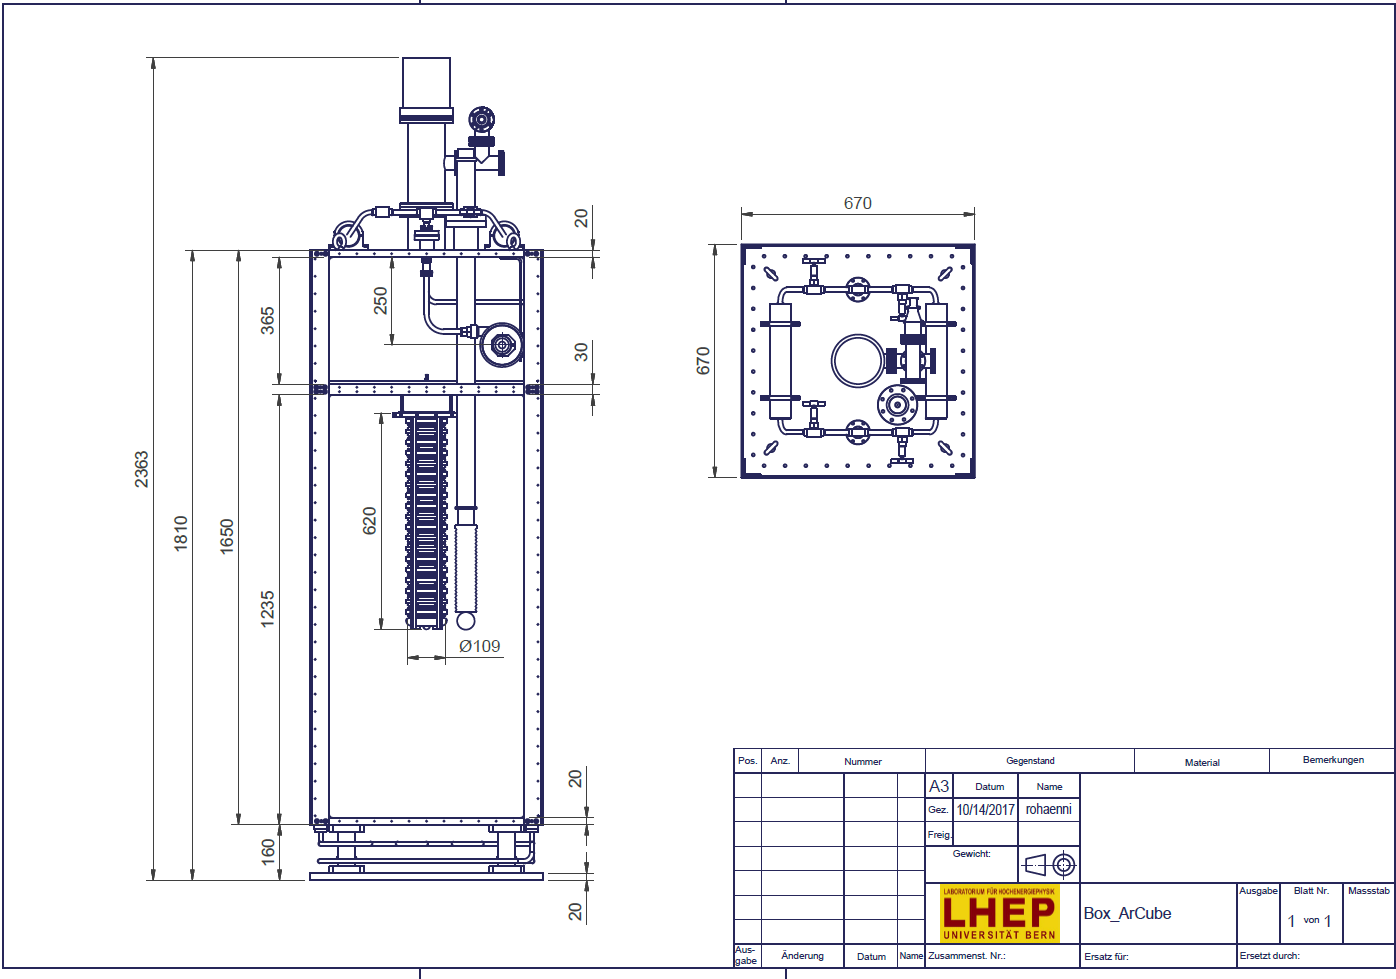
\includegraphics[width=\textwidth]{ac/2x2/dimensions}
	\caption[\AC{} \num{2 x 2} prototype module dimensions]{%
		Dimensions of a \SI{0.67 x 0.67 x 1.81}{\metre} module, equipped with the pixel demonstrator \acrshort{tpc}, for the \num{2 x 2} module \AC{} prototype at \acrshort{help}.
	}
	\label{fig:2x2_dim}
\end{figure}

\begin{figure}[htb]
	\centering
	\includegraphics[width=.66\textwidth]{ac/2x2/Viper-Module-SoftLight-4K-better_labelled}
	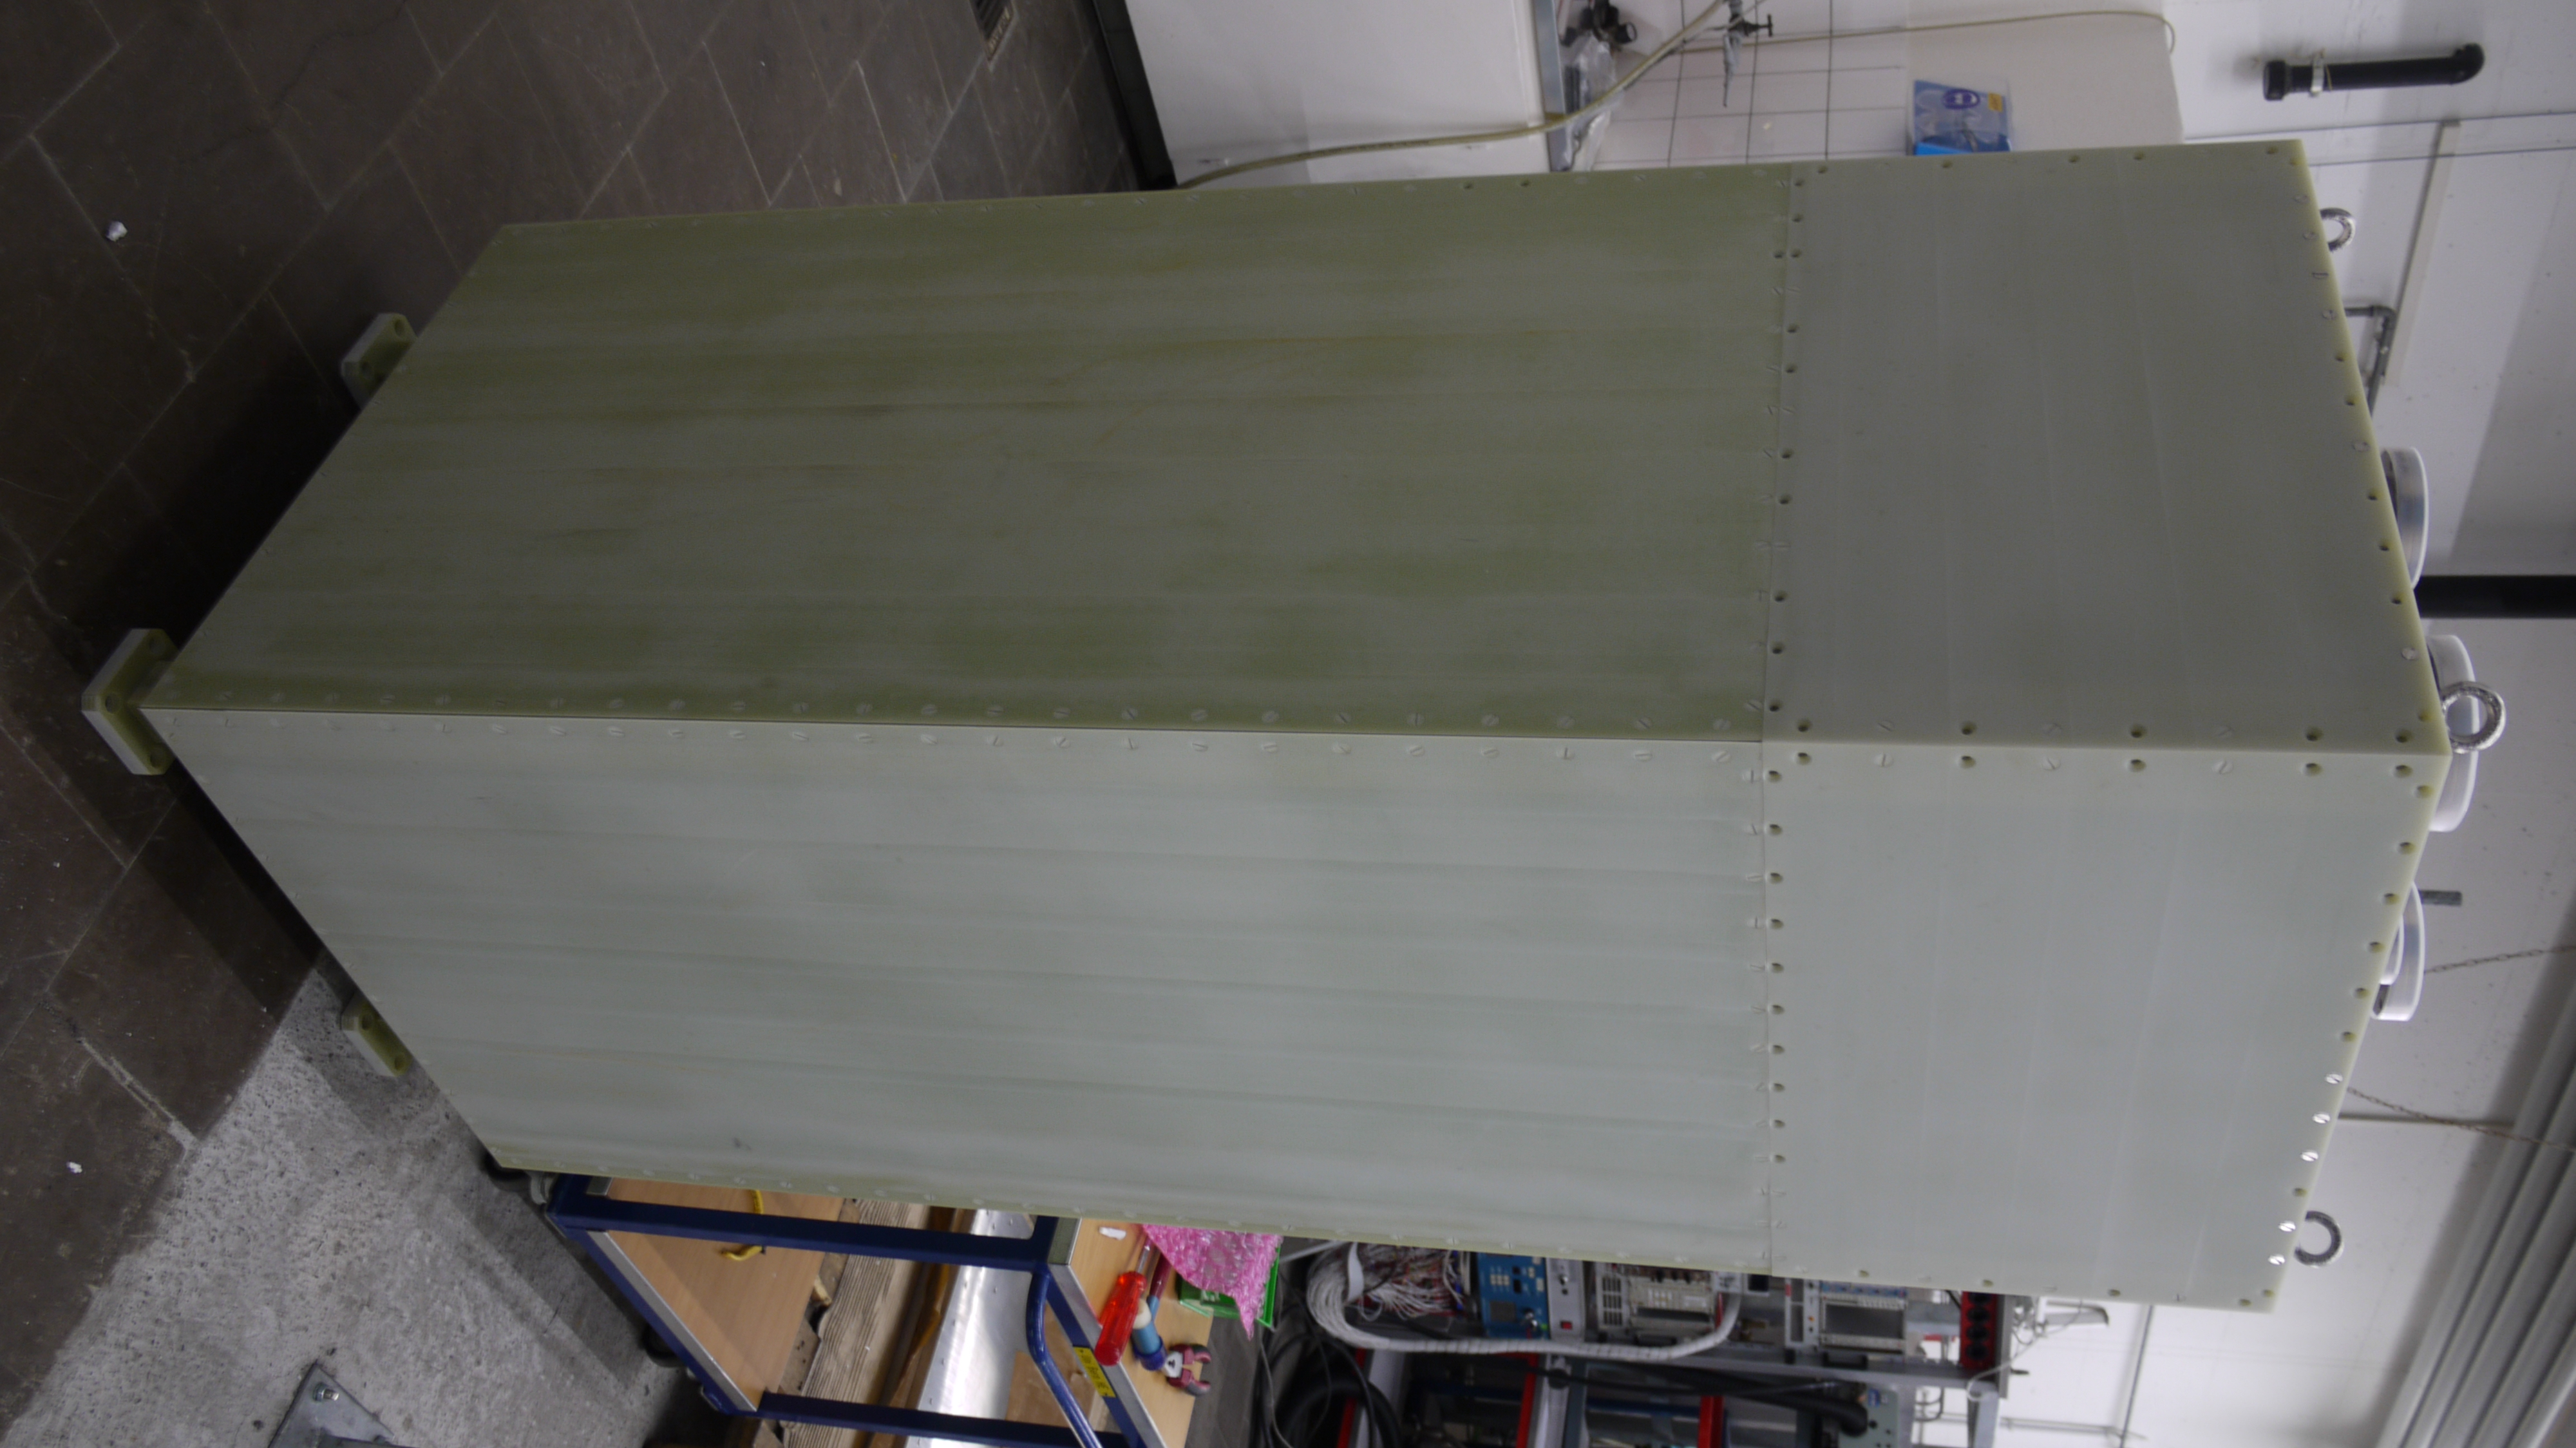
\includegraphics[height=.33\textwidth, angle=90]{ac/2x2/module_real}
	\caption[\AC{} \num{2 x 2} prototype module]{%
		Engineering drawing (left) and picture (right) of a \SI{0.67 x 0.67 x 1.81}{\metre} module, equipped with the pixel demonstrator \acrshort{tpc}, for the \num{2 x 2} module \AC{} prototype at \acrshort{help}.
	}
	\label{fig:2x2_mod}
\end{figure}

The goals of this prototype are testing the mechanical design and cryogenic systems, comparing different charge and light readout systems, and studying module insertion and extraction procedures with a focus on their influence on purity.
For comparison, one of the four modules will be equipped with a classic wire readout.
To investigate purity first tests will be performed with the \AC{} demonstrator \gls{tpc} described in Section~\ref{sec:ac_viper}.
The \gls{tpc} will be mounted inside an otherwise empty module, hanging from an intermediate support layer.
This will also serve as a first cryogenic stress-test of the module structure and \lar{} purification.

The four modules will be housed in an existing cylindrical, vacuum-insulated cryostat at \gls{help}.
An artistic view is shown in Figure~\ref{fig:ac_module-ins-ext}.
With its approximately \SI{2}{\metre} diameter by \SI{2}{\metre} height the cryostat provides a \lar{} bath volume of roughly \SI{6}{\metre\cubed}.
To fit inside the bath the modules are scaled down to a footprint of \SI{0.67 x 0.67}{\metre} and a height of \SI{1.81}{\metre}.
Instead of service volumes cooling is provided by two turbo-cooling circuits attached to the inner cryostat wall inside the insulation vacuum.
They cool the \lar{} bath via evaporation of liquid nitrogen.
The nitrogen flow has to be regulated precisely to keep the \lar{} stable and prevent it from boiling or freezing.

The height of the actual \gls{tpc} in a fully equipped module is \SI{1235}{\milli\metre}.
Due to the split-\gls{tpc} design the resulting cathode voltage required for a \SI{1}{\kilo\volt\per\centi\metre} field is below \SI{35}{\kilo\volt}.
On the bottom \SI{160}{\milli\metre} are occupied by the heat exchanger and check valves for \lar{} exchange with the bath upon insertion and extraction.
The remaining room on top of the \gls{tpc} is filled up by the \gls{hv} feedthrough, a buffer gas phase, and an optional recirculation pump.
All support structures except for the flanges at the module top and bottom are made from \emph{Amsler \& Frey HGW 2372} G10~\cite{g10}, including most of the screws.
The thickness of the side walls is \SI{10}{\milli\metre} while the flanges are made of \SI{20}{\milli\metre} stainless steel plates.
An engineering drawing of a \num{2 x 2} prototype module is given in Figure~\ref{fig:ac_module}.
It uses a \lar{} pump donated by \gls{fail} in combination with oxygen traps mounted on top of the module.

Figure~\ref{fig:2x2_dim} gives the detailed dimensions of a prototype module.
It depicts the first module, which will be equipped with the demonstrator \gls{tpc}.
For this test an internal pump salvaged from \AT{} will be used.
An engineering drawing together with a picture of the pixel demonstrator module is given in Figure~\ref{fig:2x2_mod}.

Table~\ref{tab:dune-nd_dim} gives an overview of the most important dimensions of the \num{2 x 2} module prototype at \gls{help} and the preliminary \dune{} \gls{nd} design (see Section~\ref{sec:dune-nd_ac-nd}).
In particular, the table contains a rough estimate of dead space, caused by the modular design, and the corresponding active volume fraction.
For these calculations a total charge readout thickness of \SI{20}{\milli\metre} and a total light readout thickness of \SI{5}{\milli\metre} were assumed.
The difference is caused by the fact that charge readout electronics are located directly behind the readout while the \glspl{sipm} are only mounted on the edges of the \AL{} modules.
Additionally, a few \si{\milli\metre} clearance between the anode plane and the module wall are required for convection cooling of the \larpix{} electronics.
Readout thicknesses also include the clearance between adjacent modules ($\sim{\SI{1}{\milli\metre}}$).
The resulting total fraction of active volume is \SI{87.0}{\percent} for the \num{2 x 2} module prototype.

In a first phase the \num{2 x 2} prototype will be operated in the Grosslabor of \gls{help}, taking cosmic ray data.
After a successful test of all subsystems, it is planned to be installed in a test beam at either CERN or \gls{fail} to investigate the influence of the module walls on calorimetry and tracking.

\begin{table}[htb]
	\centering
	\caption[\AC{} \num{2 x 2} prototype and \glsentryshort{dune} \glsentryshort{nd} dimensions]{%
		\AC{} dimensions for the \num{2 x 2} prototype at \acrshort{help} and the preliminary \acrshort{dune} \acrshort{nd} design.
		Charge and light readout thicknesses are given per wall, i.e.\ the resulting dead space per module is twice as big.
		Both are preliminary estimates.
		For simplicity clearance between adjacent modules is included in these numbers.
	}
	\label{tab:dune-nd_dim}
	\begin{tabu} to \textwidth {lSSs}
		\toprule
		Dimension &						{\num{2 x 2}} &			{\acrshort{nd}} &		{Unit} \\
		\midrule
		Detector size &					\num{2 x 2} &			\num{4 x 5} &			mod \\
		Module footprint &				\num{0.670 x 0.670} &	\num{1.000 x 1.000} &	\metre\squared \\
		Module height &					1.810 &					3.500 &					\metre \\
		\acrshort{tpc} height &			1.235 &					3.000 &					\metre \\
		Total \acrshort{tpc} volume &	2.218 &					60.000 &				\metre\cubed \\
		Flange thickness &				0.020 &					0.020 &					\metre \\
		Side wall thickness &			0.010 &					0.010 &					\metre \\
		Charge readout thickness &		0.020 &					0.020 &					\metre \\
		Light readout thickness &		0.005 &					0.005 & 				\metre \\
		Total dead volume &				0.289 &					5.292 &					\metre\cubed \\
		Active volume fraction &		87.0 &					91.2 &					\percent \\
		\bottomrule
	\end{tabu}
\end{table}


\section{Preliminary \AC{} \glsentrylong{nd} Design}
\label{sec:dune-nd_ac-nd}

\begin{figure}[htb]
	\centering
	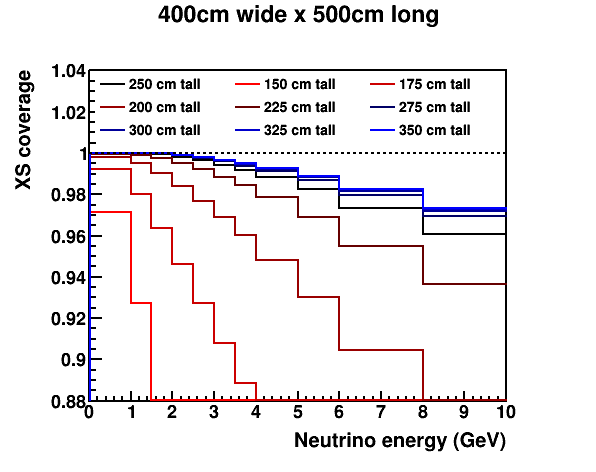
\includegraphics[width=\textwidth]{ac/dune_nd/lartpc_size_vertical}
	\caption[\AC{} \glsentryshort{dune} \glsentryshort{nd} hadron containment]{%
		Influence of the \acrshort{lartpc} size in the \acrshort{dune} \acrshort{nd} complex on hadron containment.
		Given in cross-section coverage as a function of neutrino energy.
		Horizontal dimensions are held constant at their nominal values of \SI{4 x 5}{\metre}.
		Height is indicated by colour.
		See text for explanation of cross-section coverage.~\cite{lartpcSizeChris}
	}
	\label{fig:dune-nd_lartpc-size}
\end{figure}

\begin{figure}[htb]
	\centering
	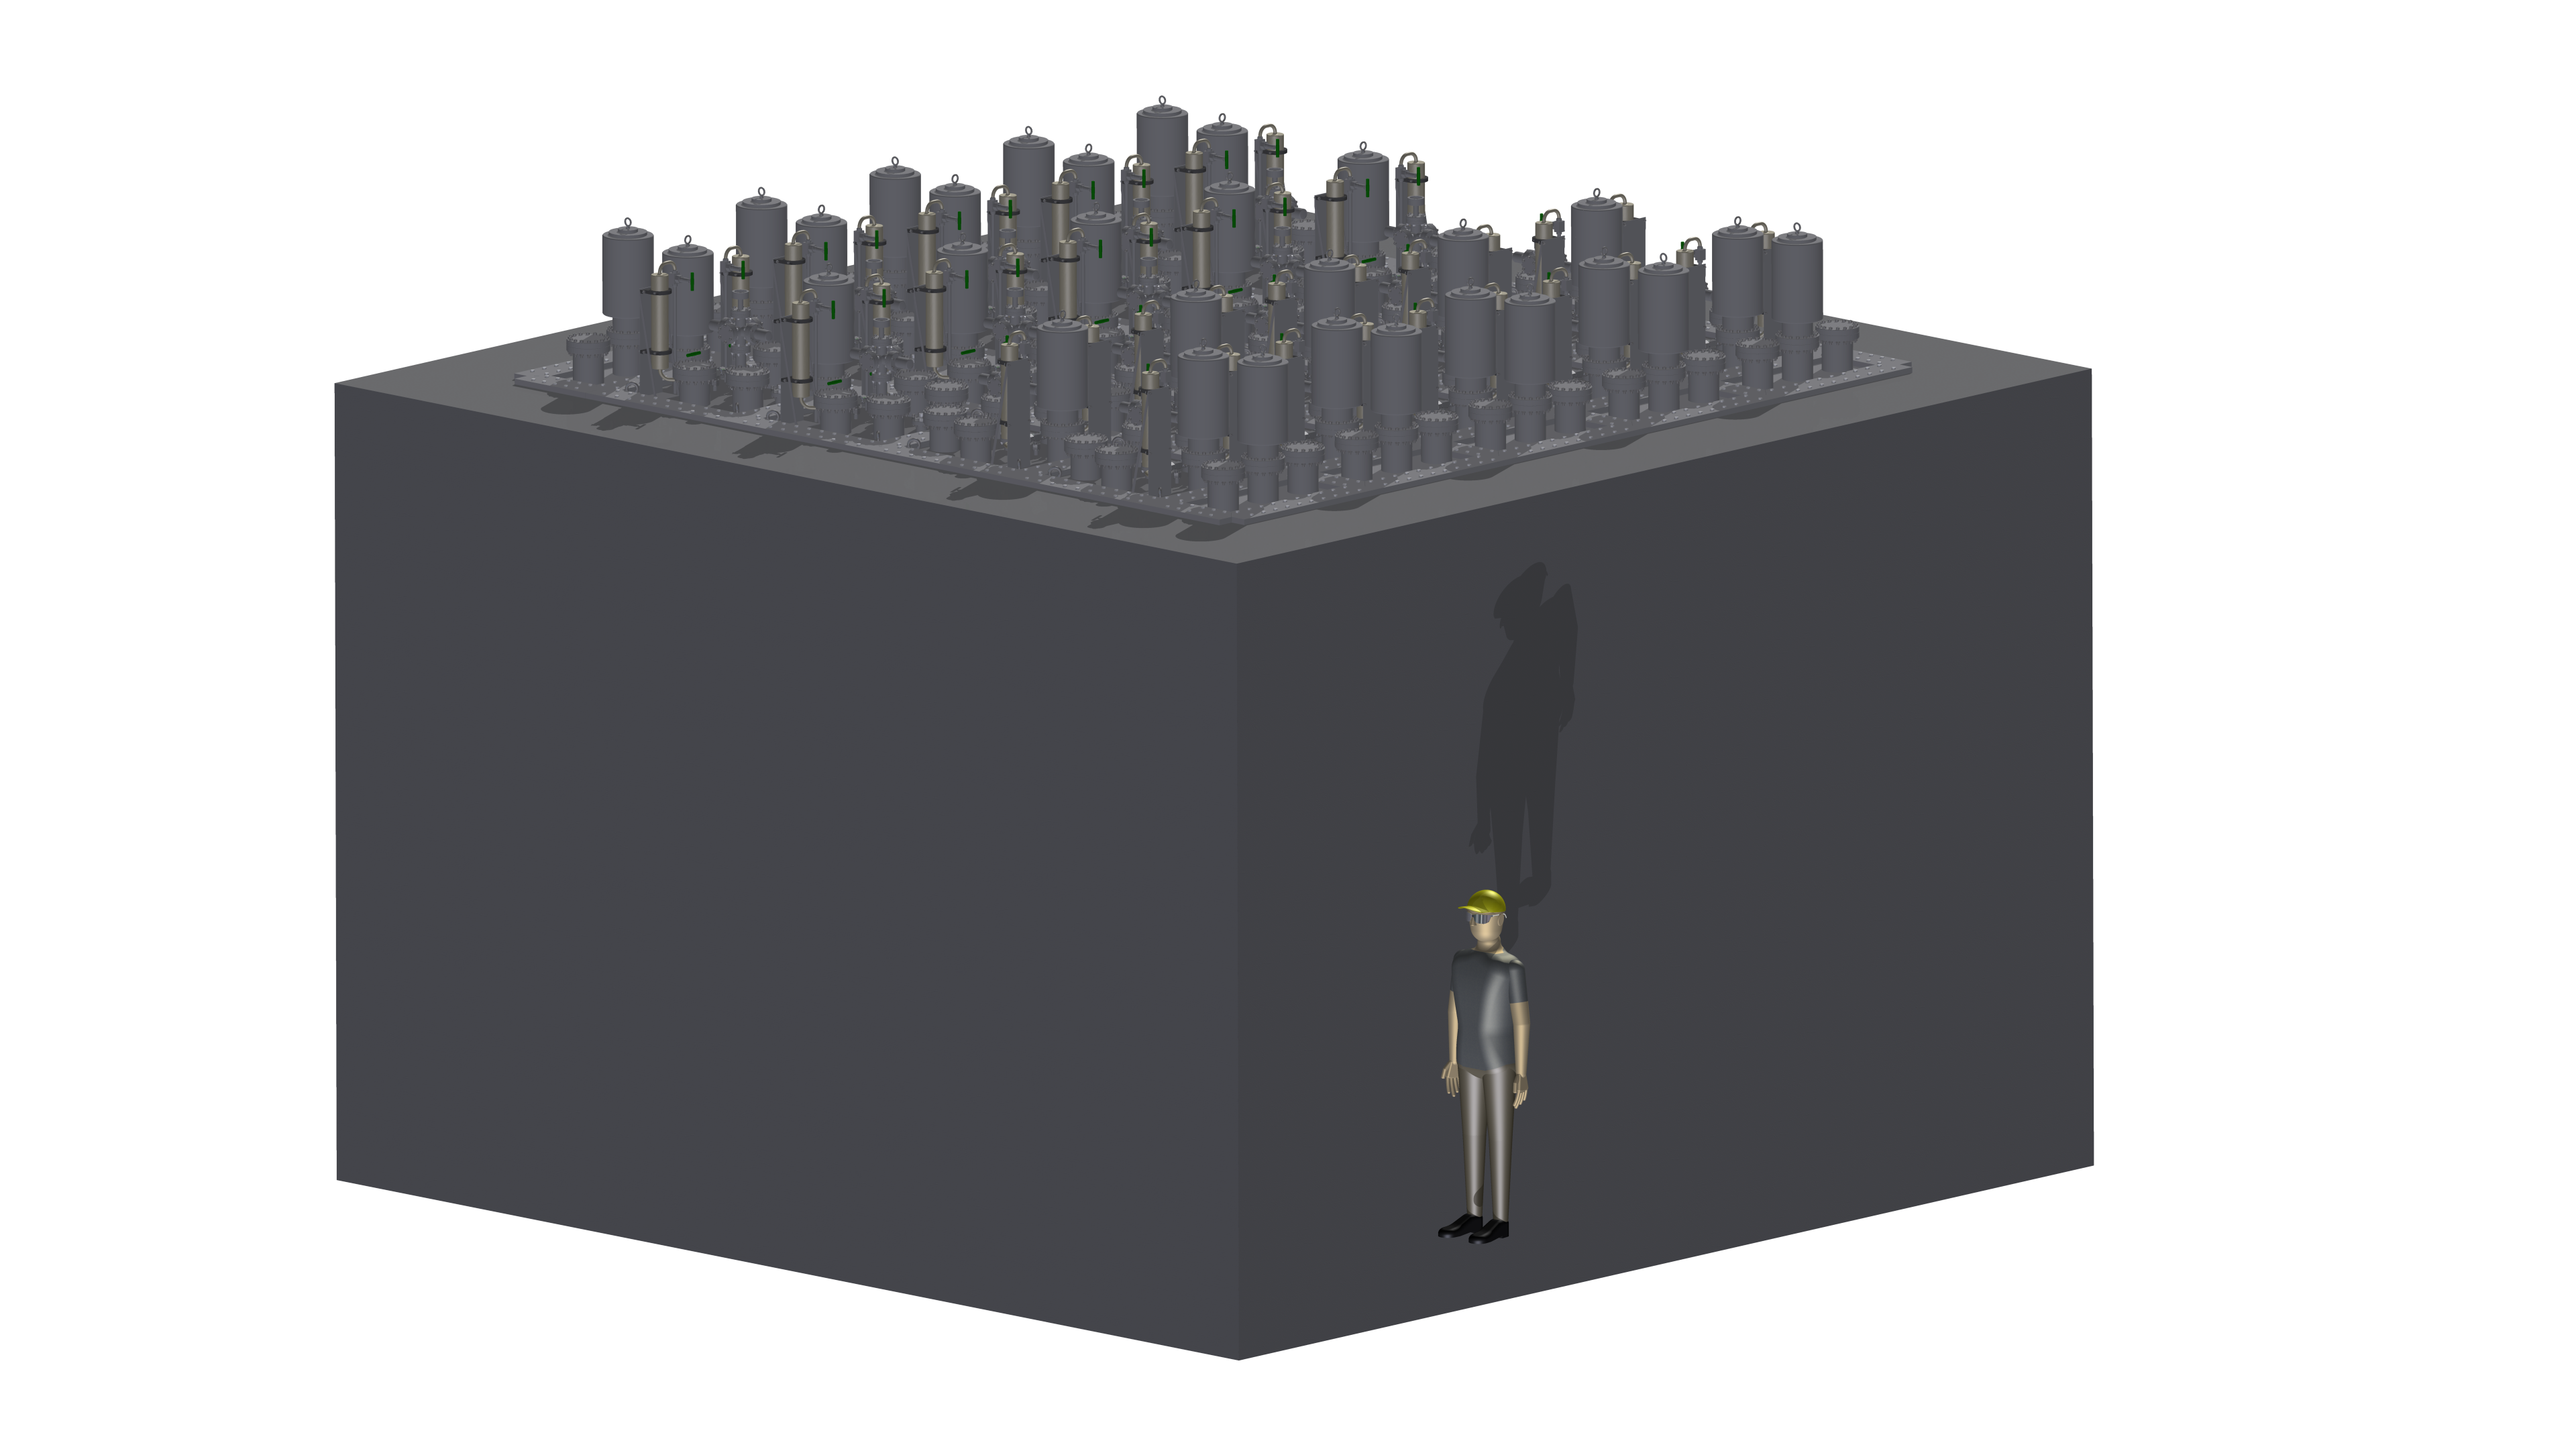
\includegraphics[width=\textwidth]{ac/dune_nd/DUNE-ND-2018}
	\caption[\AC{} \glsentryshort{dune} \glsentryshort{nd} artistic view]{%
		Artistic view of the \acrshort{dune} \acrshort{nd} \AC{} component.
		Drawn with individual pump and oxygen traps for each module.
	}
	\label{fig:dune-nd_ac}
\end{figure}

The \AC{} \gls{nd} design is based on a scaled-up version of the \num{2 x 2} module prototype design described in Section~\ref{sec:dune-nd_ac-2x2}.
Modules will have a footprint of \SI{1 x 1}{\metre} and a height of \SI{3.5}{\metre}.
Again, \SI{0.1}{\metre} at the bottom are occupied by the heat exchanger and valves while \SI{0.4}{\metre} at the top are taken up by feedthroughs and the gas phase.
This results in a \gls{tpc} size of \SI{1 x 1 x 3}{\metre}, split in two half \glspl{tpc} by a cathode at a potential of \SI{50}{\kilo\volt}.
The full detector will consist of \num{4 x 5} modules with the longer dimension in beam direction.

Detector dimensions were optimised for maximum hadron containment by means of simulations done by the neutrino group at \gls{lbnl}~\cite{lartpcSizeChris}.
While horizontal dimensions are unproblematic, the vertical \SI{3}{\metre} are at the lower limit.
According to the simulations, \SI{2.5}{\metre} would be sufficient but provide no safety margin at all.
Reducing the height by another \SI{0.25}{\metre} results in a significant loss of hadron containment already.
Figure~\ref{fig:dune-nd_lartpc-size} illustrates this by means of the cross-section coverage as a function of neutrino energy.
Cross-section coverage is similar to containment efficiency but should not be confused with the latter.
To assess the efficiency a detector of the corresponding size in the neutrino beam is simulated.
While this indeed provides a good measure of the efficiency of the detector to contain different events, it is not necessarily a good quantity to assess the required detector size.
Many events are simply not contained because of their specific location and/or orientation inside the detector.
Cross-section coverage remedies this deficiency by looking at the actual extent of the event instead of its containment at a random position inside a realistic detector.
On the other hand, an event extending through the full detector will very likely never be contained in a real detector due to the low probability of it exactly happening in the right location.
Therefore, the maximum event size needs to be selected smaller than the full detector size.
For the \gls{nd} simulation this buffer was chosen as \SI{0.5}{\metre} in all directions; i.e.\ an event can have a maximum extent of \SI{2 x 3 x 4}{\metre} to be counted as contained in a nominal size detector.
Like this cross-section coverage allows to probe for phase space regions inaccessible to a particular detector configuration.
In Figure~\ref{fig:dune-nd_lartpc-size} it can be seen that cross-section coverage decreases rapidly for detector heights below \SI{2.5}{\metre}.
A height of \SI{3}{\metre} is therefore preferable to have some buffer for yet unknown uncertainties in the simulation.

A pixel pitch of \SI{3}{\milli\metre} was chosen.
This value has been field-tested in a physics experiment, \uboone{}~\cite{uboone}, and is below the $\approx \SI{5}{\milli\metre}$ wire pitch of the \dune{} \glspl{fd}~\cite{dune4}.
The \larpix{} electronics described in Section~\ref{sec:studies_pixel-electronics} are designed to be capable of handling the data rates and power consumption expected for a \SI{3}{\milli\metre} pixel pitch \AC{} \gls{nd} component.
Therefore, a sufficient spatial resolution from a physics point of view is provided while keeping the power and data rate demands on the readout electronics under control.

Inspired by the design of the \dune{} \SI{35}{\tonne} prototype at \gls{fail}~\cite{dune4} the \lar{} bath is held in a foam-insulated membrane cryostat.
The outer support structure is a \SI{0.3}{\metre} thick steel-reinforced concrete layer, followed by a \SI{0.4}{\metre} thick polyurethane foam layer for thermal insulation.
Inside of this is a \SI{2}{\milli\metre} thick stainless steel membrane sealing the \lar{} bath from the environment.
There are several other support layers, all of which with a thickness of $\sim{\SI{1}{\milli\metre}}$, with a more detailed description in~\cite{dune4}.
The total thickness of the cryostat wall amounts to \num{2.88} radiation lengths.
Cooling is provided by \num{10} uninstrumented \SI{0.5 x 1}{\metre} service volumes equipped with cryocoolers, arranged along the two detector edges parallel to beam direction.
The total required cryostat footprint is therefore \SI{5 x 5}{\metre}.

Table~\ref{tab:dune-nd_dim} gives an overview of the most important \AC{} \gls{nd} dimensions, in comparison to the \num{2 x 2} module prototype at \gls{help}.
Due to the bigger modules the total fraction of active volume is increased to \SI{91.2}{\percent}.
Drift direction is perpendicular to beam direction to reduce the hit rate on single pixels.
If drift direction is parallel to beam direction, particle tracks highly parallel to drift direction lead to a very high rate on single channels, potentially leading to a buffer overflow and thus data loss in the \larpix{} chip.
In addition, power dissipation increases proportionally to the pixel hit rate due to the smart zero suppression scheme of \larpix{}.
Another advantage is that dead space in beam direction between adjacent modules will only be \SI{30}{\milli\metre} due to the very slim dimensions of \AL{}.
Figure~\ref{fig:dune-nd_ac} shows an artistic view of the \AC{} \gls{nd} component.